\documentclass{article}
\usepackage{tkz-graph}
\usepackage{paralist}
\pagestyle{empty}
\usetikzlibrary{patterns}

\begin{document}

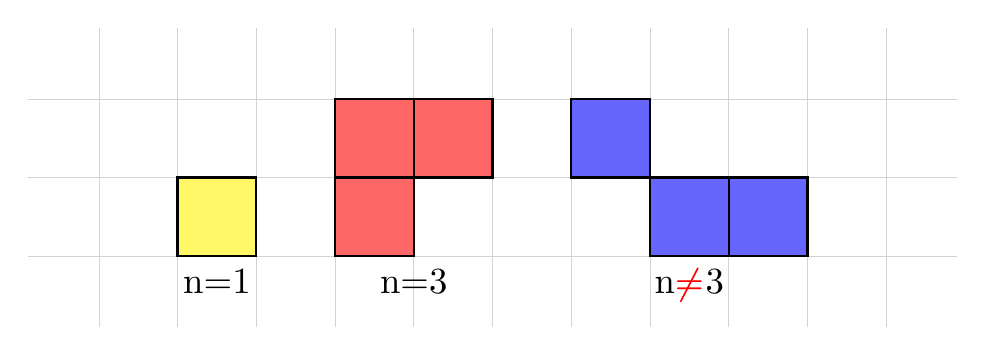
\begin{tikzpicture}
\draw[step=1cm,gray!35,very thin] (-5.9,3.1) grid (5.9,6.9);

\filldraw[yellow!60, draw=black, thick] (-4,4) rectangle (-3,5);
\draw (-3.5,4) -- (-3.5,4) node[anchor=north, scale=1.33] {n=1};

\filldraw[red!60, draw=black, thick] (-2,4) rectangle (-1,5);
\filldraw[red!60, draw=black, thick] (-2,5) rectangle (-1,6);
\filldraw[red!60, draw=black, thick] (-1,5) rectangle (0,6);
\draw (-1,4) -- (-1,4) node[anchor=north, scale=1.33] {n=3};

\filldraw[blue!60, draw=black, thick] (1,5) rectangle (2,6);
\filldraw[blue!60, draw=black, thick] (2,4) rectangle (3,5);
\filldraw[blue!60, draw=black, thick] (3,4) rectangle (4,5);
\draw (2.5,4) -- (2.5,4) node[anchor=north, scale=1.33] {n \, 3};
\filldraw[red] (2.5,4) -- (2.5,4) node[anchor=north, scale=1.33] {$\ne$};
\filldraw[red] (2.5,4) -- (2.5,4) node[anchor=north, scale=1.33] {$\ne$};

\end{tikzpicture}

\end{document}